\subsection{Lab5: Modulación BPSK en GRC}

%*********************
\begin{frame}{}

\pgfdeclareimage[width=\paperwidth,height=\paperheight]{bg}{imagenes/fondo_lab}
\setbeamertemplate{background}{\pgfuseimage{bg}}

\bfseries{\textrm{\LARGE Lab5\\ \Large Flujo de datos digitales\\BPSK en GRC}}
\raggedright
\end{frame}
%********************

%--------------------------------------------------------------------------------------------
\begin{frame}{Flujo de datos digitales BPSK}

\pgfdeclareimage[width=\paperwidth,height=\paperheight]{bg}{imagenes/fondo3}
\setbeamertemplate{background}{\pgfuseimage{bg}}

\justifying
Cómo convertir un flujo de datos digitales en una señal analógica de banda base utilizando un filtro FIR interpolador
\\
\begin{figure}
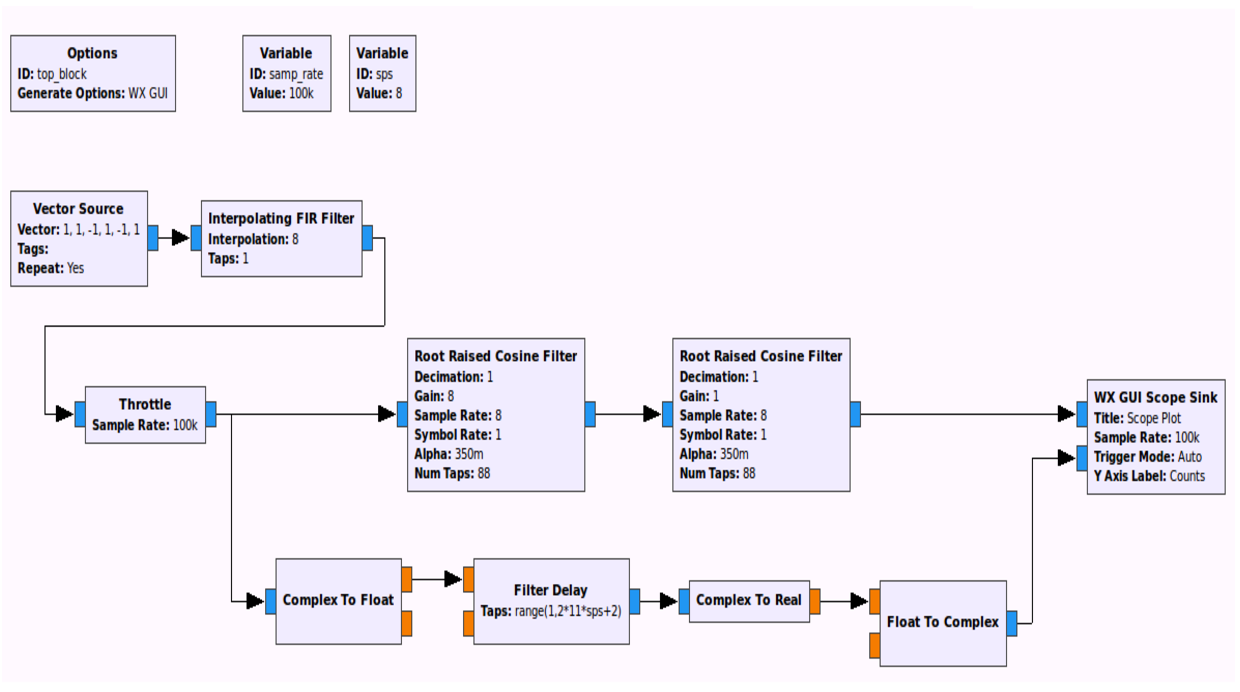
\includegraphics[width=.9\textwidth]{parte1/lab5/pdf/lab5_1.pdf}
\end{figure}
\end{frame}
%---------------------------------------------------------------------------
%\includegraphics[scale=1]{../imagenes/descarga.jpeg} 

\begin{frame}{Flujo de datos digitales BPSK}
\begin{figure}
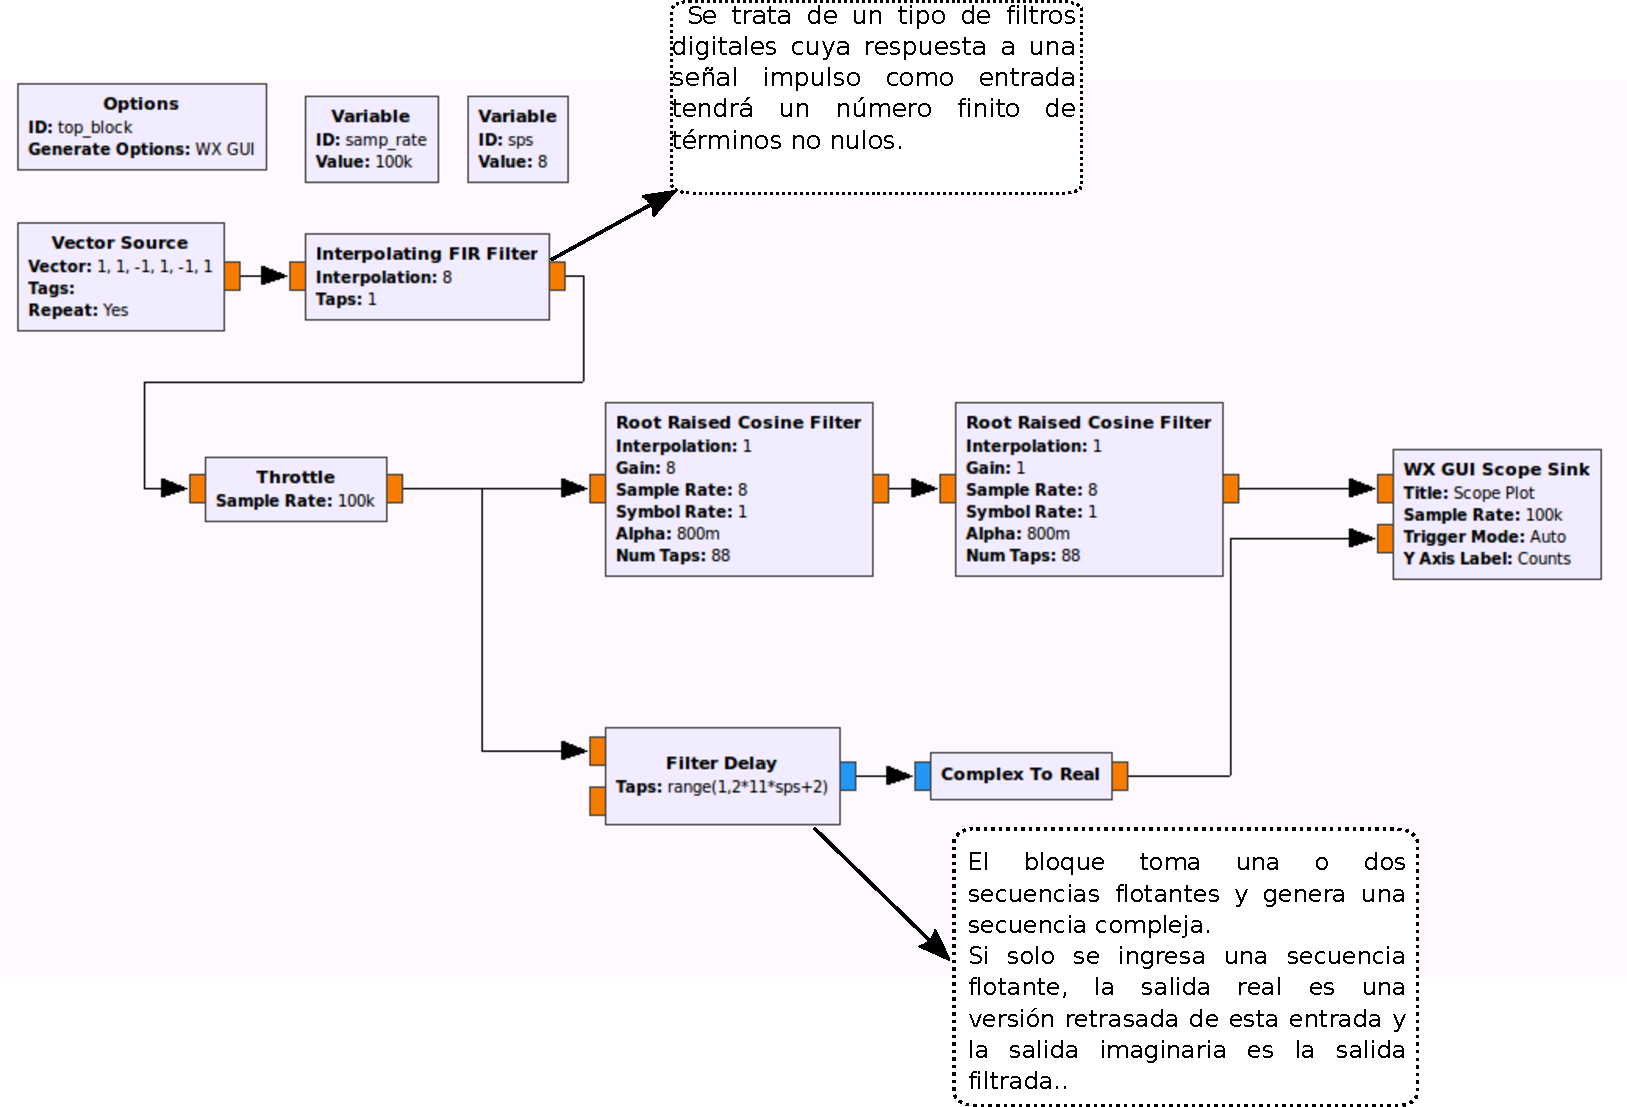
\includegraphics[width=.9\textwidth]{parte1/lab5/pdf/lab5_2.pdf}
\end{figure}
\end{frame}
%--------------------------------------------------------------------------------------
\begin{frame}{Flujo de datos digitales BPSK}
\frametitle{Flujo de datos digitales BPSK}
\framesubtitle{Filtros FIR}
Un filtro FIR es aquel que tiene una respuesta finita al impulso y que se caracterizan por ser sistemas no recursivos.Un filtro FIR de orden L se describe mediante la ecuación en diferencias:\\
\centering
$$y\left ( n \right )=a_{0}x\left ( n \right )+a_{1}x\left (n-1  \right )+a_{2}\left ( n-2 \right )+...+a_{L}x\left ( n-L \right )$$
\\
\justifying
Donde la secuencia $a_k$ son los coeficientes del filtro. A partir de esta
ecuación en diferencias puede obtenerse la función de transferencia del
filtro en el dominio de Z.\\
\centering
 $$F\left ( z \right )=\sum_{k=0}^{L-1}a\left [ k \right ]z^{-1}$$
\\
\justifying
En este tipo de filtrado no existe retroalimentación. Además, la respuesta
al impulso $H\left (w \right)$, es de duración finita ya que si la entrada se mantiene en cero durante $L$ periodos consecutivos la salida también será cero. 
\end{frame}
%---------------------------------------------------------------------------------------

\begin{frame}{Flujo de datos digitales BPSK}
\begin{figure}
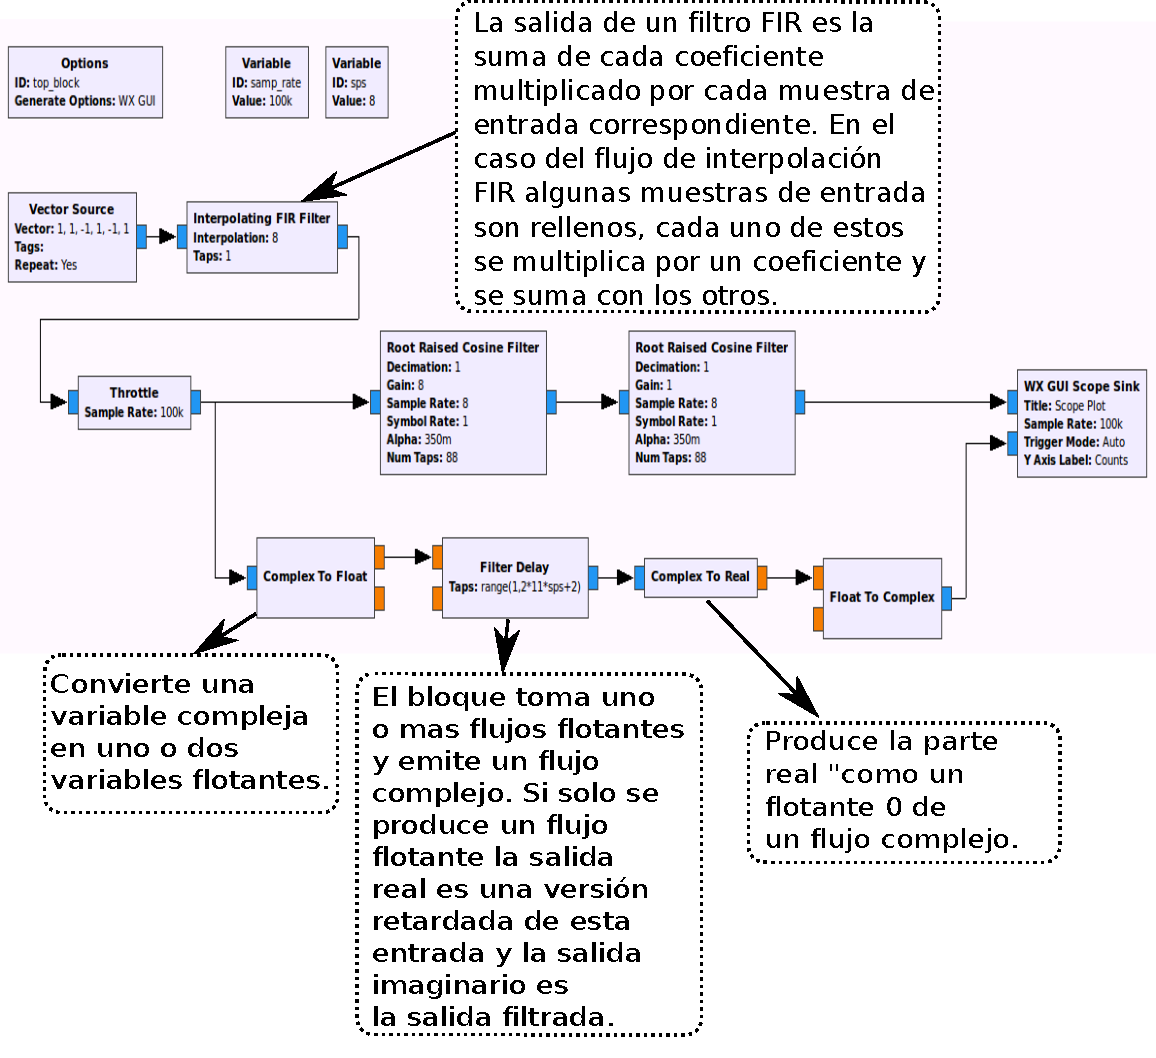
\includegraphics[width=.9\textwidth]{parte1/lab5/pdf/lab5_3.pdf}
\end{figure}
\end{frame}

%--------------------------------------------------------------------------------

\begin{frame}{Flujo de datos digitales BPSK}
\frametitle{Flujo de datos digitales BPSK}
\framesubtitle{¿Qué es y para que se utiliza el Root Raised Cosine Filter?}
\justifying
Uno de los principales inconvenientes de todas las formas de onda de la señal es que, aunque pueden controlar muy bien las emisiones de energía dentro del ancho de banda de interés, envían cantidades relativamente altas de energía de esta. Una forma práctica de reducir los lóbulos laterales del espectro de las señales de navegación podría ser usar un filtro de coseno realsado (RCF), ya que tiene un ancho de banda limitado. El filtro de coseno realsado es un caso particular del filtro Nyquist. Los pulsos de Nyquist (filtros) son pulsos que no producen interferencia entre símbolos (ISI) en el momento del muestreo.
\end{frame}
%-----------------------------------------------------------------------------------
\begin{frame}{Flujo de datos digitales BPSK}
\begin{figure}
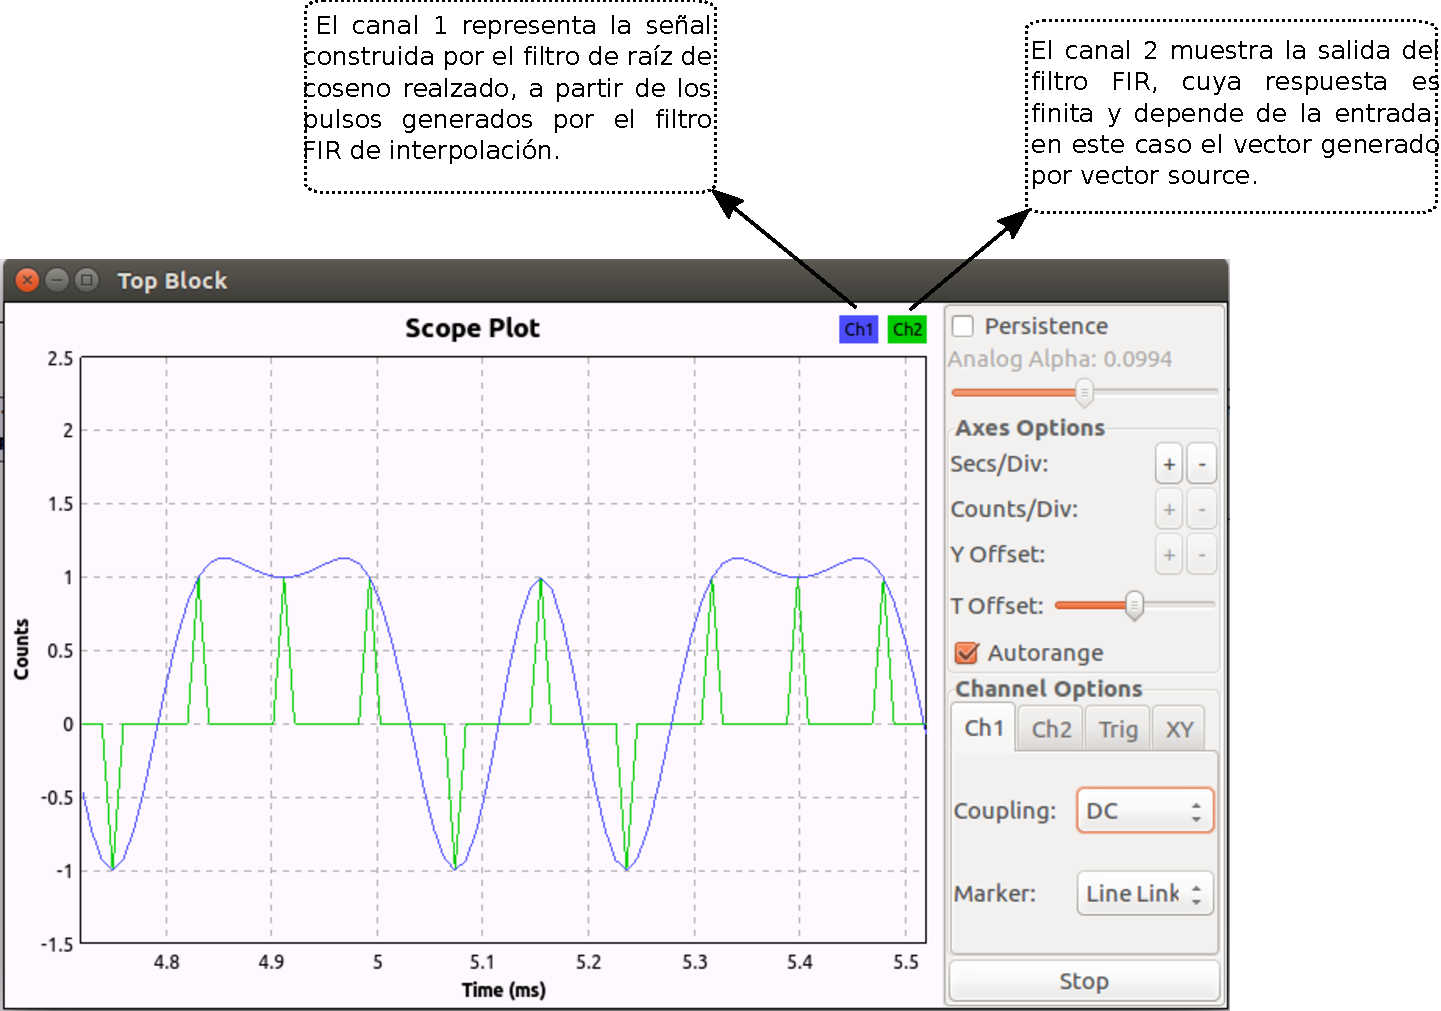
\includegraphics[width=.9\textwidth]{parte1/lab5/pdf/lab5_4.pdf}
\end{figure}
\end{frame}
%-------------------------------------------------------------------------------------------
\begin{frame}{Flujo de datos digitales BPSK}
\justifying
Puesto que el diagrama de constelación es un método de representación en el plano complejo de los estados de símbolo en términos de amplitud y fase en los esquemas de modulación digital,sera necesario para ver este diagrama  utilizar un flujo de datos complejos, como se ve acontinuación:
\begin{figure}
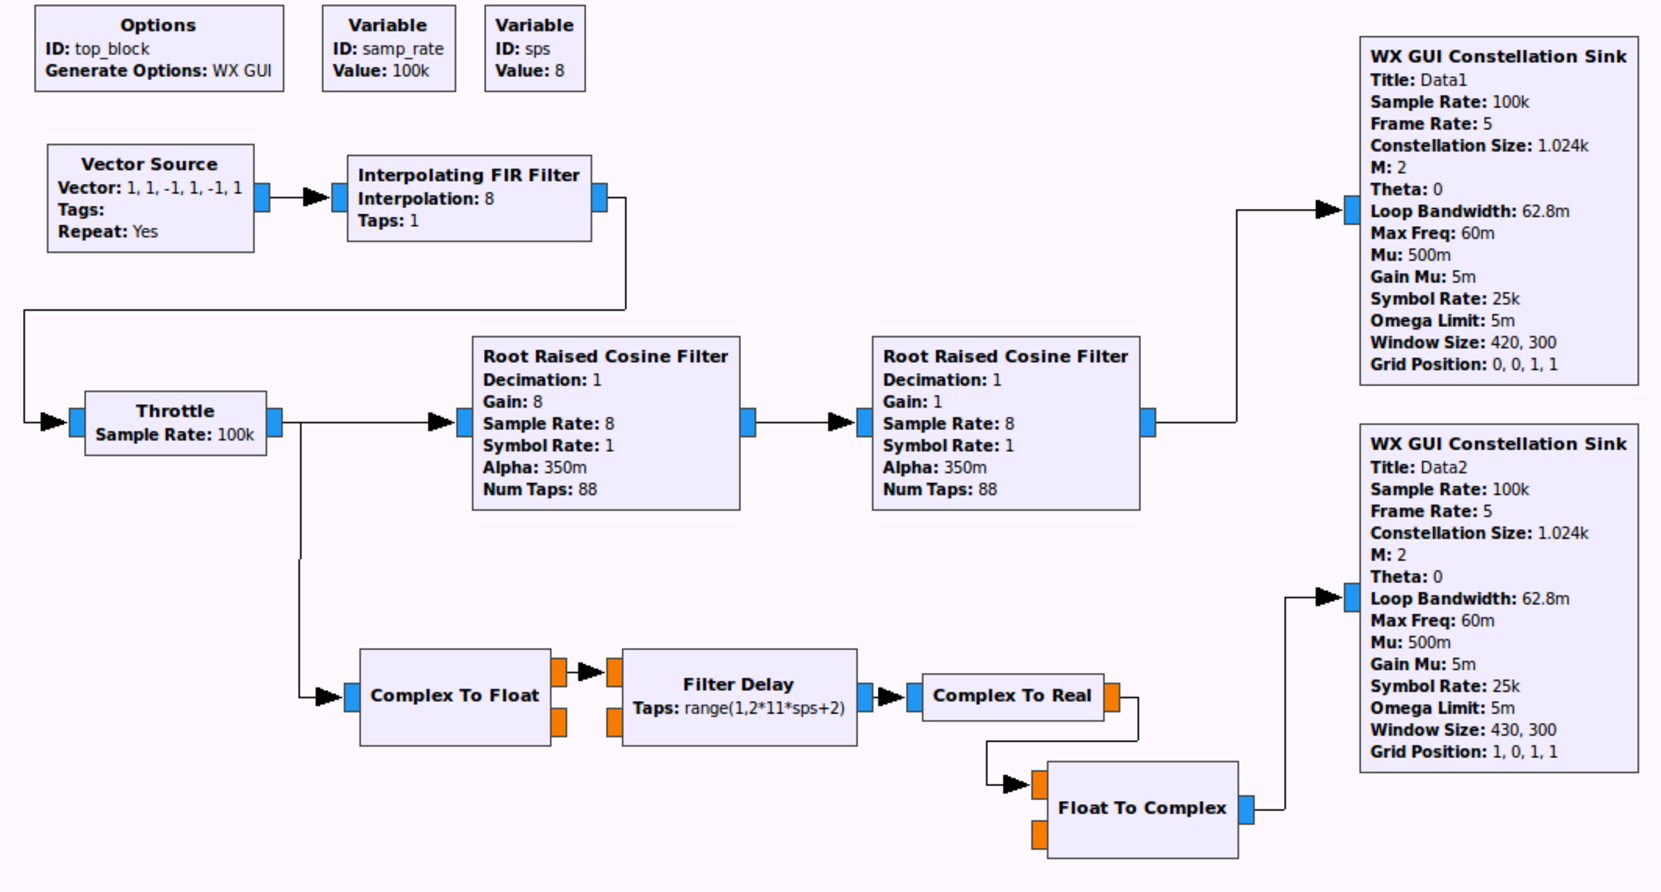
\includegraphics[width=.9\textwidth]{parte1/lab5/pdf/lab5_5.pdf}
\end{figure}
\end{frame}
%------------------------------------------------------------------------------------------
\begin{frame}{Flujo de datos digitales BPSK}
\begin{figure}
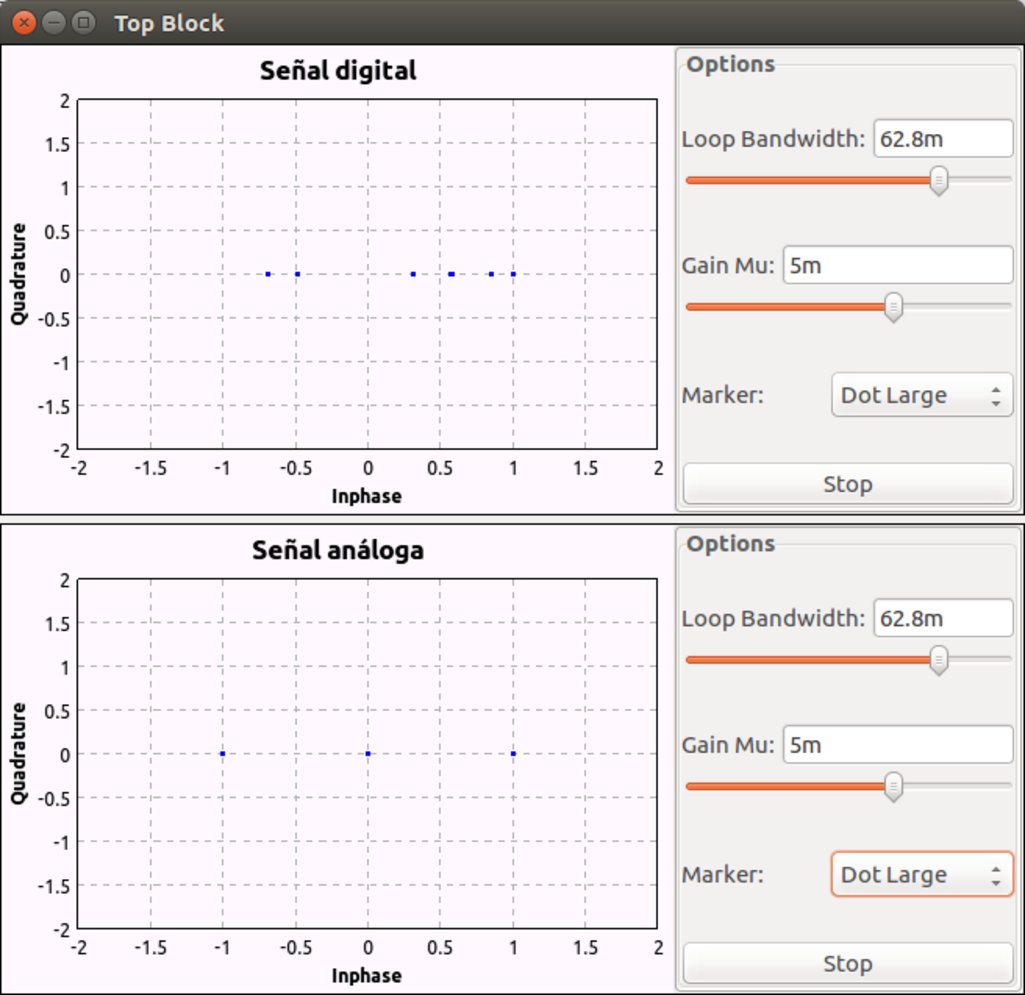
\includegraphics[width=.6\textwidth]{parte1/lab5/pdf/lab5_6.pdf}
\end{figure}
\end{frame}
\subsubsection{actividad_1_lab_5}

%*********************
\begin{frame}
\pgfdeclareimage[width=\paperwidth,height=\paperheight]{bg}{imagenes/fondo_seccion}
\setbeamertemplate{background}{\pgfuseimage{bg}}

\definecolor{greenU}{RGB}{212,202,72}
\setbeamercolor{block body}{fg=Black,bg=greenU}
\begin{block}{}
\centering
\vspace{8mm}
\Large{Actividades}
\vspace{8mm}
\end{block}
\end{frame}
%********************

%--------------------------------------------------------------------------------------------
\begin{frame}{Flujo de datos digitales BPSK}
\pgfdeclareimage[width=\paperwidth,height=\paperheight]{bg}{imagenes/fondo3}
\setbeamertemplate{background}{\pgfuseimage{bg}}

\frametitle{Flujo de datos digitales BPSK}
\framesubtitle{Actividad}
¿Qué efectos produce el parámetro $\alpha$ del fltro de raíz de coseno realzado sobre la señal y el ancho de banda?\\
\begin{itemize}
\item Grafique en un bloque de WX GUI FFT Sink la salida del segundo bloque de Root Raised Cosine Filter.Recuerde antes convertir los datos de flotantes a tipo complejo.     
\item Realice cambios al parámetro $\alpha$ del bloque Root Raised Cosine Filter, y observe los cambios en el FFT Plot y en el Scope Plot.
\end{itemize}

\end{frame}
%----------------------------------------------------------------------------
 